\documentclass[10pt]{article}
\usepackage[utf8]{inputenc}
\usepackage[T1]{fontenc}
\usepackage{amsmath}
\usepackage{amsfonts}
\usepackage{amssymb}
\usepackage[version=4]{mhchem}
\usepackage{stmaryrd}
\usepackage{graphicx}
\usepackage[export]{adjustbox}
\graphicspath{ {./images/} }
\usepackage{caption}

\begin{document}
\captionsetup{singlelinecheck=false}
\section*{FINAL JEE-MAIN EXAMINATION - JANUARY, 2023 \\
 (Held On Wednesday \(\mathbf{2 5}^{\text {th }}\) January, 2023) \\
 TIME : 3: 00 PM to 6:00 PM}
\section*{CHEMISTRY}
\section*{SECTION-A}
\begin{enumerate}
  \setcounter{enumi}{30}
  \item Match List I with List II
\end{enumerate}

\begin{center}
\begin{tabular}{|l|l|l|l|}
\hline
 & List I &  & List II \\
\hline
A. & Cobalt catalyst & I. & \(\left(\mathrm{H}_{2}+\mathrm{Cl}_{2}\right)\) production \\
\hline
B. & Syngas & II. & Water gas production \\
\hline
C. & Nickel catalyst & III. & Coal gasification \\
\hline
D. & Brine solution & IV. & Methanol production \\
\hline
\end{tabular}
\end{center}

Choose the correct answer from the options given below :-\\
(1) A-IV, B-I, C-II, D-III\\
(2) A-IV, B-III, C-I, D-II\\
(3) A-II, B-III, C-IV, D-I\\
(4) A-IV, B-III, C-II, D-I

Official Ans. by NTA (4)\\
Allen Ans. (4)\\
Sol. Cobalt catalyst \(\rightarrow\) Methanol production\\
Syn gas \(\rightarrow\) Coal gasification\\
\(\left(\mathrm{C}_{\text {(Red hot coke) }}+\mathrm{H}_{2} \mathrm{O}(\mathrm{g}) \rightarrow \mathrm{CO}+\mathrm{H}_{2}\right)\)\\
Nickel catalyst \(\rightarrow\) Water gas production\\
Brine solution \(\rightarrow\) Production\\
(aq. NaCl\() \quad\binom{\mathrm{H}_{2} \rightarrow \text { Cathode }}{\mathrm{Cl}_{2} \rightarrow \text { anode }}\)\\
32. Given below are two statements :-

Statement I :- In froth floatation method a rotating paddle agitates the mixture to drive air out of it.

Statement II :- Iron pyrites are generally avoided for extraction of iron due to environmental reasons. In the light of the above statements, choose the correct answer from the options given below :-\\
(1) Both Statement I and Statement II are true

\section*{TEST PAPER WITH SOLUTION}
(2) Statement I is false but Statement II is true\\
(3) Statement I is true but Statement II is false\\
(4) Both Statement I and Statement II are false

Official Ans. by NTA (2)\\
Allen Ans. (2)\\
Sol. In froth floatation method a rotating paddle draws in air and stirs the pulp.\\
33. Which of the following represents the correct order of metallic character of the given elements?\\
(1) \(\mathrm{Si}<\mathrm{Be}<\mathrm{Mg}<\mathrm{K}\)\\
(2) \(\mathrm{Be}<\mathrm{Si}<\mathrm{Mg}<\mathrm{K}\)\\
(3) \(\mathrm{K}<\mathrm{Mg}<\mathrm{Be}<\mathrm{Si}\)\\
(4) \(\mathrm{Be}<\mathrm{Si}<\mathrm{K}<\mathrm{Mg}\)

Official Ans. by NTA (1)\\
Allen Ans. (1)\\
Sol. Metallic character increases down the group and decreases along the period.\\
34. Given below are two statements, one is labelled as Assertion A and the other is labelled as Reason R

Assertion A :- The alkali metals and their salts impart characteristic colour to reducing flame.

Reason R :- Alkali metals can be detected using flame tests.

In the light of the above statements, choose the most appropriate answer form the options given below\\
(1) Both A and R are correct but R is NOT the correct explanation of A .\\
(2) A is correct but R is not correct.\\
(3) A is not correct but R is correct\\
(4) Both A and R are correct and R is the correct explanation of A .

Official Ans. by NTA (3)\\
Allen Ans. (3)\\
Sol. The alkali metals and their salts impart characteristic colour to oxidizing flame.\\
35. What is the mass ratio of ethylene glycol ( \(\mathrm{C}_{2} \mathrm{H}_{6} \mathrm{O}_{2}\), molar mass \(=62 \mathrm{~g} / \mathrm{mol})\) required for making 500 g\\
of 0.25 molal aqueous solution and 250 mL of 0.25 molar aqueous solution ?\\
(1) \(1: 1\)\\
(2) \(3: 1\)\\
(3) \(2: 1\)\\
(4) \(1: 2\)

\section*{Official Ans. by NTA (3)}
Allen Ans. (3)\\
Sol. Assume : Mass of solvent \(\approx\) Mass of solution\\
Case I :-\\
\(0.25=\frac{\mathrm{W}_{1}}{62} \times \frac{1000}{500}\)\\
Case II :-\\
\(0.25=\frac{\mathrm{W}_{2}}{62} \times \frac{1000}{250}\)\\
\(\frac{\mathrm{W}_{1}}{\mathrm{~W}_{2}}=\frac{2}{1}\)\\
36. Statement I :- Dipole moment is a vector quantity and by convention it is depicted by a small arrow with tail on the negative centre and head pointing towards the positive centre.

Statement II :- The crossed arrow of the dipole moment symbolizes the direction of the shift of charges in the molecules.

In the light of the above statements, choose the most appropriate answer from the options given below :-\\
(1) Both Statement I and Statement II are correct.\\
(2) Statement I is incorrect but Statement II is correct.\\
(3) Both Statement I and Statement II are incorrect.\\
(4) Statement I is correct but Statement II is incorrect.

Official Ans. by NTA (4)\\
Allen Ans. (4)\\
Sol. Statement II : The corssed arrow symbolises the direction of the shift of electron density in the molecule.\\
37. Given below are two statements, one is labelled as Assertion A and the other is labelled as Reason R Assertion A :- Butylated hydroxyl anisole when added to butter increases its shelf life.

Reason R :- Butylated hydroxyl anisole is more reactive towards oxygen than food.

In the light of the above statements, choose the most appropriate answer from the options given below :-\\
(1) Both A and R are correct and R is the correct explanation of A .\\
(2) A is correct but R is not correct.\\
(3) A is not correct but R is correct.\\
(4) Both A and R are correct but R is NOT the correct explanation of A .

Official Ans. by NTA (1)\\
Allen Ans. (1)\\
Sol. Butylated hydroxyl anisole is an antioxidant.\\
38. A. Ammonium salts produce haze in atmosphere.\\
B. Ozone gets produced when atmospheric oxygen reacts with chlorine radicals.\\
C. Polychlorinated biphenyls act as cleansing solvents.\\
D. 'Blue baby' syndrome occurs due to the presence of excess of sulphate ions in water.

Choose the correct answer from the options given below :-\\
(1) A, B and C only\\
(2) B and C only\\
(3) A and D only\\
(4) A and C only

Official Ans. by NTA (4)\\
Allen Ans. (4)\\
Sol. B. \(\dot{\mathrm{C}}+\mathrm{O}_{3} \longrightarrow \mathrm{O}_{2}+\mathrm{Cl} \dot{\mathrm{O}}\)\\
D. 'Blue baby' syndrome occurs due to the presence of excess of nitrate ions in water.\\
39. Match List I with List II

\begin{center}
\begin{tabular}{|l|l|l|l|}
\hline
 & List I (Amines) &  & \begin{tabular}{l}
List II \\
\(\left(\mathrm{pK}_{\mathrm{b}}\right)\) \\
\end{tabular} \\
\hline
A. & Aniline & I. & 3.25 \\
\hline
B. & Ethanamine & II. & 3.00 \\
\hline
C. & N-Ethylethanamine & III. & 9.38 \\
\hline
D. & N, N-Diethylethanamine & IV. & 3.29 \\
\hline
\end{tabular}
\end{center}

Choose the correct answer from the options given below :-\\
(1) A-I, B-IV, C-II, D-III\\
(2) A-III, B-II, C-I, D-IV\\
(3) A-III, B-II, C-IV, D-I\\
(4) A-III, B-IV, C-II, D-I

Official Ans. by NTA (4)\\
Allen Ans. (4)\\
Sol.\\
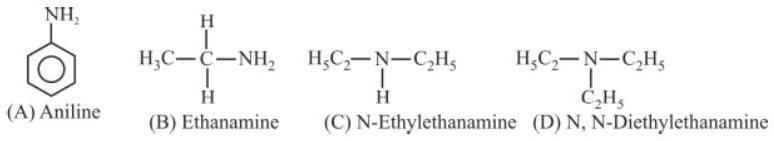
\includegraphics[max width=\textwidth, center]{2025_10_02_f0bf008abd968cf9b89ag-3(2)}

Basic Strength \(\alpha \frac{1}{\mathrm{pK}_{\mathrm{b}}}\)\\
Order for \(\mathrm{pK}_{\mathrm{b}}: \mathrm{A}>\mathrm{B}>\mathrm{D}>\mathrm{C}\)\\
40. Which one among the following metals is the weakest reducing agent ?\\
(1) K\\
(2) Rb\\
(3) Na\\
(4) Li

Official Ans. by NTA (3)\\
Allen Ans. (3)\\
Sol. Sodium have lowest oxidation potential in alkali metals. Hence it is weakest reducing agent among alkali metals.\\
41. Match List I with List II.

\begin{center}
\begin{tabular}{|l|l|l|l|}
\hline
 & \begin{tabular}{l}
List I \\
Isomeric pairs \\
\end{tabular} &  & \begin{tabular}{l}
List II \\
Type of \\
isomers \\
\end{tabular} \\
\hline
A. & \begin{tabular}{l}
Propanamine and N- \\
Methylethanamine \\
\end{tabular} & I. & Metamers \\
\hline
B. & Hexan-2-one and & II. & Positional \\
\hline
\end{tabular}
\end{center}

\begin{center}
\begin{tabular}{|l|l|l|l|}
\hline
 & Hexan-3-one &  & isomers \\
\hline
C. & \begin{tabular}{l}
Ethanamide and \\
Hydroxyethanimine \\
\end{tabular} & III. & \begin{tabular}{l}
Functional \\
isomers \\
\end{tabular} \\
\hline
D. & \begin{tabular}{l}
o-nitrophenol and p- \\
nitrophenol \\
\end{tabular} & IV. & Tautomers \\
\hline
\end{tabular}
\end{center}

Choose the correct answer from the options given below :-\\
(1) A-III, B-IV, C-I, D-II\\
(2) A-IV, B-III, C-I, D-II\\
(3) A-II, B-III, C-I, D-IV\\
(4) A-III, B-I, C-IV, D-II

Official Ans. by NTA (4)\\
Allen Ans. (4)\\
Sol. A. Propanamine N-Methylethanamine\\
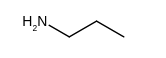
\includegraphics{smile-58f0738b8e07431592427e7b99443ba7ca24c13c}\\
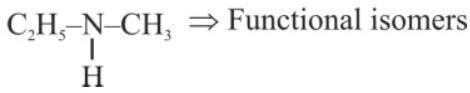
\includegraphics[max width=\textwidth, center]{2025_10_02_f0bf008abd968cf9b89ag-3(1)}\\
B. Hexan-2-one

Hexan-3-one\\
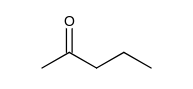
\includegraphics{smile-33f515a48c52af2f8866ef87e6e9be48a1f8a2e2}\\
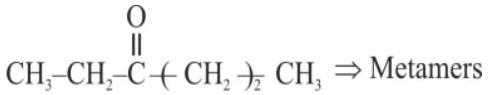
\includegraphics[max width=\textwidth, center]{2025_10_02_f0bf008abd968cf9b89ag-3}\\
C. Ethanamide

Hydroxyethanimine\\
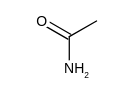
\includegraphics{smile-be72fb54504545214cf94a0f91682d30dc77c803}\\
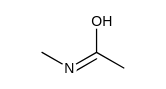
\includegraphics{smile-3b85956f804b3db77fdd9aa2d7592d466ba1ee2d}\\
D. o-Nitrophenol\\
p-nitrophenol\\
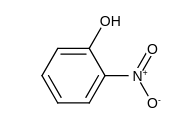
\includegraphics{smile-96f45913643d4339970b516436b8c1591a676131}\\
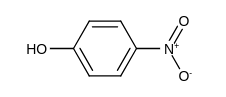
\includegraphics{smile-8c9cc737c2682856fdc16d19aa8fae093f7eeed3}\\
\(\Rightarrow\) Positional isomers\\
42. Match List I with List II

\begin{center}
\begin{tabular}{|l|l|l|l|}
\hline
 & \begin{tabular}{l}
List I (Name of \\
polymer) \\
\end{tabular} &  & List II (Uses) \\
\hline
A. & Glyptal & I. & Flexible pipes \\
\hline
B. & Neoprene & II. & Synthetic wool \\
\hline
C. & Acrilan & III. & Paints and Lacquers \\
\hline
D. & LDP & IV. & Gaskets \\
\hline
\end{tabular}
\end{center}

Choose the correct answer from the options given below :-\\
(1) A-III, B-II, C-IV, D-I\\
(2) A-III, B-IV, C-II, D-I\\
(3) A-III, B-IV, C-I, D-II\\
(4) A-III, B-I, C-IV, D-II

Official Ans. by NTA (2)\\
Allen Ans. (2)\\
43. Given below are two statements, one is labelled as Assertion A and the other is labelled as Reason R

Assertion A :- Carbon forms two important oxides -CO and \(\mathrm{CO}_{2} . \mathrm{CO}\) is neutral whereas \(\mathrm{CO}_{2}\) is acidic in nature.

Reason R :- \(\mathrm{CO}_{2}\) can combine with water in a limited way to form carbonic acid, while CO is sparingly soluble in water.

In the light of the above statements, choose the most appropriate answer from the options given below :-\\
(1) Both A and R are correct but R is NOT the correct explanation of A .\\
(2) Both A and R are correct and R is the correct explanation of A .\\
(3) A is not correct but R is correct.\\
(4) A is correct but R is not correct.

\section*{Official Ans. by NTA (2)}
\section*{Allen Ans. (2)}
Sol. The oxide which form acid on dissolving in water is acidic oxide.\\
44. Potassium dichromate acts as a strong oxidizing agent in acidic solution. During this process, the oxidation state changes from\\
(1) +3 to +1\\
(2) +6 to +3\\
(3) +2 to +1\\
(4) +6 to +2

\section*{Official Ans. by NTA (2)}
\section*{Allen Ans. (2)}
Sol. \(14 \mathrm{H}^{+}+6 \mathrm{e}^{-}+\underset{\underset{+6}{\mathrm{Cr}_{2}} \mathrm{O}_{7}^{-2}}{\underline{+6}} \longrightarrow \underset{\underline{+3}}{2 \mathrm{Cr}^{+3}}+7 \mathrm{H}_{2} \mathrm{O}\)\\
45. When the hydrogen ion concentration \(\left[\mathrm{H}^{+}\right]\)changes by a factor of 1000, the value of pH of the solution\\
\(\_\_\_\_\) .\\
(1) increases by 1000 units\\
(2) decreases by 3 units\\
(3) decreases by 2 units\\
(4) increases by 2 units

\section*{Official Ans. by NTA (4)}
\section*{Allen Ans. (2)}
Sol. \(\quad \Delta\left[\mathrm{H}^{+}\right]=1000\)

\[
\Delta \mathrm{pH}=-\log \Delta\left[\mathrm{H}^{+}\right]=-\log 10^{3}
\]

\[
=-3
\]

\begin{enumerate}
  \setcounter{enumi}{45}
  \item Match List I with List II
\end{enumerate}

\begin{center}
\begin{tabular}{|l|l|l|l|}
\hline
 & \begin{tabular}{l}
List I \\
Coordination entity \\
\end{tabular} &  & \begin{tabular}{l}
List II \\
Wavelength of light absorbed in nm \\
\end{tabular} \\
\hline
A. & \(\left[\mathrm{CoCl}\left(\mathrm{NH}_{3}\right)_{5}\right]^{2+}\) & I. & 310 \\
\hline
B. & \(\left[\mathrm{Co}\left(\mathrm{NH}_{3}\right)_{6}\right]^{3+}\) & II. & 475 \\
\hline
C. & \(\left[\mathrm{Co}(\mathrm{CN})_{6}\right]^{3-}\) & III. & 535 \\
\hline
D. & \(\left[\mathrm{Cu}\left(\mathrm{H}_{2} \mathrm{O}\right) 4^{4}\right]^{2+}\) & IV. & 600 \\
\hline
\end{tabular}
\end{center}

Choose the correct answer from the options given below :-\\
(1) A-IV, B-I, C-III, D-II\\
(2) A-III, B-II, C-I, D-IV\\
(3) A-III, B-I, C-II, D-IV\\
(4) A- II, B-III, C-IV, D-I

Official Ans. by NTA (2)\\
Allen Ans. (2)

\section*{Sol.}
\begin{center}
\begin{tabular}{|l|l|l|l|}
\hline
 & \begin{tabular}{l}
List I \\
Coordination entity \\
\end{tabular} &  & \begin{tabular}{l}
List II \\
Wavelength of light absorbed in nm \\
\end{tabular} \\
\hline
A. & \(\left[\mathrm{CoCl}\left(\mathrm{NH}_{3}\right)_{5}\right]^{2+}\) & I. & 535 \\
\hline
B. & \(\left[\mathrm{Co}\left(\mathrm{NH}_{3}\right)_{6}\right]^{3+}\) & II. & 475 \\
\hline
C. & \(\left[\mathrm{Co}(\mathrm{CN})_{6}\right]^{3-}\) & III. & 310 \\
\hline
D. & \(\left[\mathrm{Cu}\left(\mathrm{H}_{2} \mathrm{O}\right)_{4}\right]^{2+}\) & IV. & 600 \\
\hline
\end{tabular}
\end{center}

\(\mathrm{E}=\frac{\mathrm{hc}}{\lambda} \Rightarrow \mathrm{E} \propto \frac{1}{\lambda}\)\\
\(\Rightarrow \Delta(\mathrm{CFSE}) \propto \frac{1}{\lambda_{\text {absorb }}} \propto\) strength of ligand.\\
47. Find out the major product from the following reaction.\\
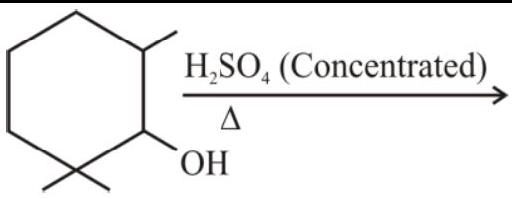
\includegraphics[max width=\textwidth, center]{2025_10_02_f0bf008abd968cf9b89ag-5}

(1)\\
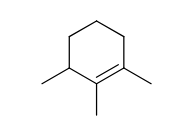
\includegraphics{smile-b52a67b07ad8b0c47926166ddd43393ceb60bca5}

(2)\\
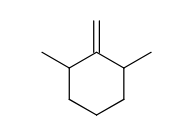
\includegraphics{smile-1d76d220c7d8c26135eacb16462e81bcdcdd0bb8}

(3)\\
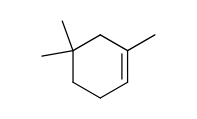
\includegraphics{smile-fde8014a79cc3fa0fe8145a0918e8ba9b8a19f71}

(4)\\
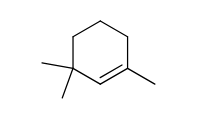
\includegraphics{smile-e28d885466d1d4c7c74cad363dc66636072597e4}

Official Ans. by NTA (1)\\
Allen Ans. (1)\\
Sol.

\begin{figure}[h]
\begin{center}
  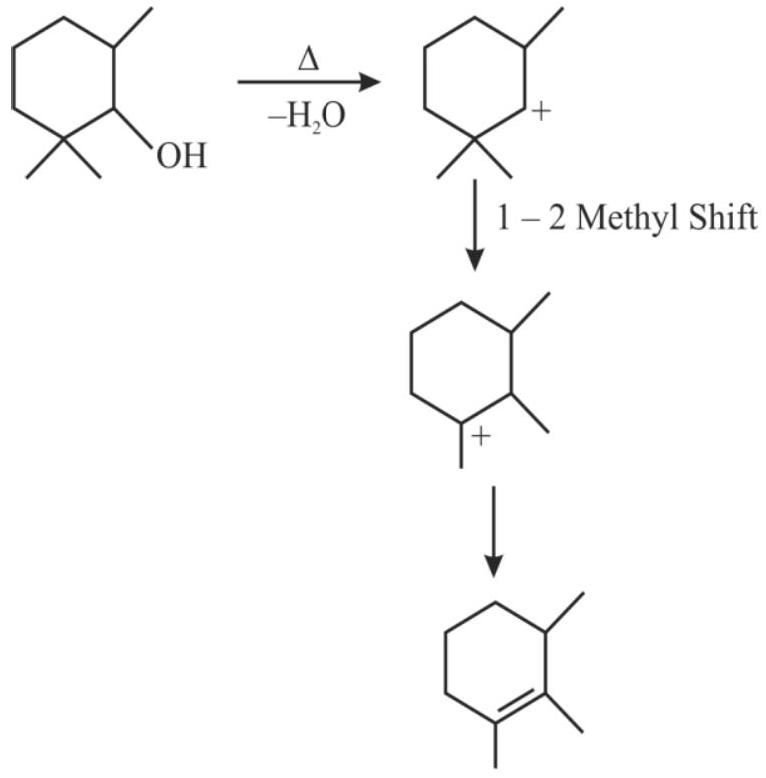
\includegraphics[width=\textwidth]{2025_10_02_f0bf008abd968cf9b89ag-5(3)}
\captionsetup{labelformat=empty}
\caption{Thermodynamically controlled product}
\end{center}
\end{figure}

Official Ans. by NTA (2)\\
Allen Ans. (2)

Sol.\\
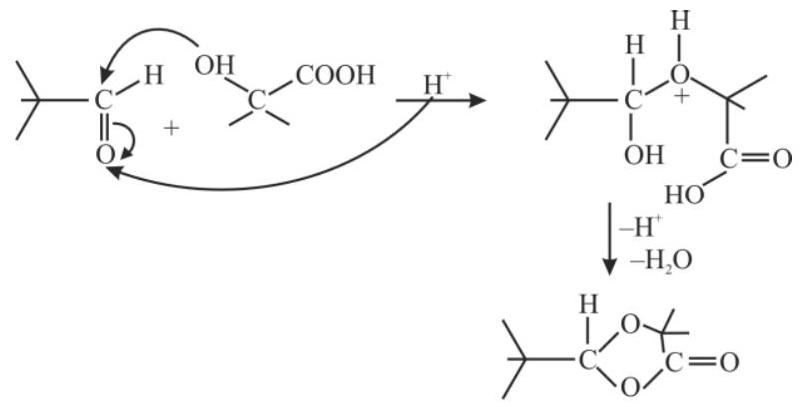
\includegraphics[max width=\textwidth, center]{2025_10_02_f0bf008abd968cf9b89ag-5(1)}\\
48. 'A' in the given reaction is\\
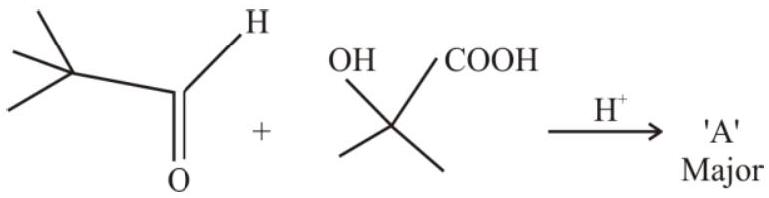
\includegraphics[max width=\textwidth, center]{2025_10_02_f0bf008abd968cf9b89ag-5(2)}

(1)\\
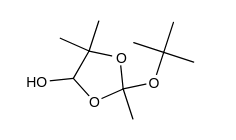
\includegraphics{smile-ca999ca5d2f377916f45b85dacf310e937155aae}

(2)\\
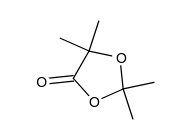
\includegraphics{smile-5eaf716ed5495fc376f24834fc22b20fa4cf6822}

(3)\\
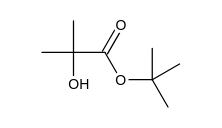
\includegraphics{smile-de100e24985157a82e0948270526d30116475531}

(4)\\
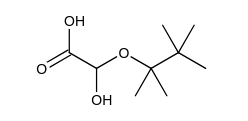
\includegraphics{smile-02b79727535de71b20b632ba5801c5ee9f376212}\\
49. The isomeric deuterated bromide with molecular formula \(\mathrm{C}_{4} \mathrm{H}_{8} \mathrm{DBr}\) having two chiral carbon atoms is\\
(1) 2-Bromo-1-deuterobutane\\
(2) 2-Bromo-2-deuterobutane\\
(3) 2-Bromo-3-deuterobutane\\
(4) 2-Bromo-1-deutero-2-methylpropane

Official Ans. by NTA (3)\\
Allen Ans. (3)

Sol.\\
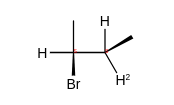
\includegraphics{smile-c064bbb1dac75a3525b086df03cf45858f26110b}\\
50. A chloride salt solution acidified with dil. \(\mathrm{HNO}_{3}\) gives a curdy white precipitate, [A], on addition of \(\mathrm{AgNO}_{3}\). [A] on treatment with \(\mathrm{NH}_{4} \mathrm{OH}\) gives a clear solution, B.\\
(1) \(\mathrm{H}\left[\mathrm{AgCl}_{3}\right]\) \& \(\left[\mathrm{Ag}\left(\mathrm{NH}_{3}\right)_{2}\right] \mathrm{Cl}\)\\
(2) \(\mathrm{H}\left[\mathrm{AgCl}_{3}\right] \&\left(\mathrm{NH}_{4}\right)\left[\mathrm{Ag}(\mathrm{OH})_{2}\right]\)\\
(3) \(\mathrm{AgCl} \&\left[\mathrm{Ag}\left(\mathrm{NH}_{3}\right)_{2}\right] \mathrm{Cl}\)\\
(4) \(\mathrm{AgCl} \&\left(\mathrm{NH}_{4}\right)\left[\mathrm{Ag}(\mathrm{OH})_{2}\right]\)

Official Ans. by NTA (3)\\
Allen Ans. (3)\\
Sol. \(\mathrm{Cl}^{-}+\mathrm{AgNO}_{3} \longrightarrow \mathrm{AgCl}\)\\
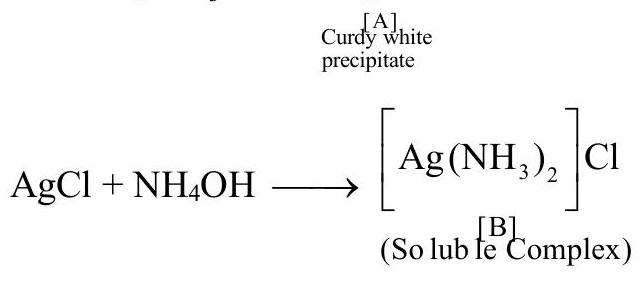
\includegraphics[max width=\textwidth, center]{2025_10_02_f0bf008abd968cf9b89ag-6}

\section*{SECTION-B}
\begin{enumerate}
  \setcounter{enumi}{50}
  \item The number of given orbitals which have electron density along the axis is \(\_\_\_\_\)\\
\(\mathrm{p}_{\mathrm{x}}, \mathrm{p}_{\mathrm{y}}, \mathrm{p}_{\mathrm{z}}, \mathrm{d}_{\mathrm{xy}}, \mathrm{d}_{\mathrm{yz}}, \mathrm{d}_{\mathrm{xz}}, \mathrm{d}_{\mathrm{z}^{2}}, \mathrm{~d}_{\mathrm{x}^{2}-\mathrm{y}^{2}}\)\\
Official Ans. by NTA (5.00)\\
Allen Ans. (5.00)\\
Sol. \(p_{x}, p_{y}, p_{z}, d_{z^{2}} \& d_{x^{2}-y^{2}}\) are axial orbitals.52.\\
Number of compounds giving (i) red colouration with ceric ammonium nitrate and also\\
(ii) positive iodoform test from the following is\\
\(\_\_\_\_\)\\
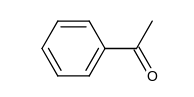
\includegraphics{smile-adc806336c454f488c8a7a7fb4559418d9eeec0c}\\
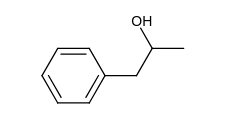
\includegraphics{smile-e7bb5e8722b6ee996fd2ebb917dd385bb9e91497}\\
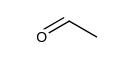
\includegraphics{smile-f8a6d92c85f590d3644d30487e76ad88e2163049}\\
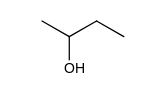
\includegraphics{smile-d4efcbc68d916727be63f5f75348bf606db19242}\\
,\\
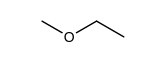
\includegraphics{smile-8e33d0bc9dc81e17713bba684a2f687852793498}\\
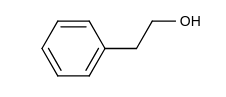
\includegraphics{smile-05b81a86cc3607c8f805ff353f876014242b03d6}\\
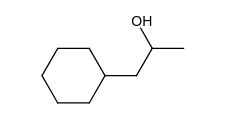
\includegraphics{smile-45a4dfbcd31c3582d1ab66c597a7ae0c05639579}\\
,\\
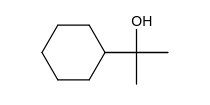
\includegraphics{smile-7bed8fa48c7352ff8ca51981b7d79dcfd6519399}
\end{enumerate}

Official Ans. by NTA (3.00)\\
Allen Ans. (3.00)

Sol.\\
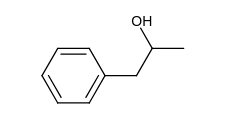
\includegraphics{smile-f0abb3d9415ed49928ca5c7d8510a9c6acafb6a3}\\
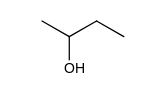
\includegraphics{smile-a11d8ff7c2e312d5326b91f1febee0f85f4200b7}\\
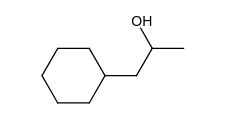
\includegraphics{smile-c82d14fedc8c09147c90578b3180e7cdd8066a4d}\\
53. The number of pairs of the solution having the same value of the osmotic pressure from the following is \(\_\_\_\_\) .\\
(Assume 100\% ionization)\\
A. \(0.500 \mathrm{M} \mathrm{C}_{2} \mathrm{H}_{5} \mathrm{OH}(\mathrm{aq})\) and \(0.25 \mathrm{M} \mathrm{KBr}(\mathrm{aq})\)\\
B. \(0.100 \mathrm{M} \mathrm{K}_{4}\left[\mathrm{Fe}(\mathrm{CN})_{6}\right](\mathrm{aq})\) and 0.100 M \(\mathrm{FeSO}_{4}\left(\mathrm{NH}_{4}\right)_{2} \mathrm{SO}_{4}(\mathrm{aq})\)\\
C. \(0.05 \mathrm{M} \mathrm{K}_{4}\left[\mathrm{Fe}(\mathrm{CN})_{6}\right](\mathrm{aq})\) and 0.25 M NaCl (aq)\\
D. \(0.15 \mathrm{M} \mathrm{NaCl}(\mathrm{aq})\) and \(0.1 \mathrm{M} \mathrm{BaCl}_{2}(\mathrm{aq})\)\\
E. \(0.02 \mathrm{M} \mathrm{KCl} . \mathrm{MgCl}_{2} .6 \mathrm{H}_{2} \mathrm{O}(\mathrm{aq})\) and 0.05 M \(\mathrm{KCl}(\mathrm{aq})\)

Official Ans. by NTA (4.00)\\
Allen Ans. (4.00)\\
Sol. \(\pi=\mathrm{iCRT}\)\\
\(\pi \propto \mathrm{iC}\)\\
\(A, B, D\) and \(E\) have same value of osmatic pressure.\\
54. 28.0 L of \(\mathrm{CO}_{2}\) is produced on complete combustion of 16.8 L gaseous mixture of ethene and methane at \(25^{\circ} \mathrm{C}\) and 1 atm . Heat evolved during the combustion process is \(\_\_\_\_\) kJ .

Given : \(\Delta \mathrm{H}_{\mathrm{C}}\left(\mathrm{CH}_{4}\right)=-900 \mathrm{~kJ} \mathrm{~mol}^{-1}\)\\
\(\Delta \mathrm{H}_{\mathrm{C}}\left(\mathrm{C}_{2} \mathrm{H}_{4}\right)=-1400 \mathrm{~kJ} \mathrm{~mol}^{-1}\)\\
Official Ans. by NTA (925.00)\\
Allen Ans. (847.00)\\
Sol. Let, Volume of \(\mathrm{C}_{2} \mathrm{H}_{4}\) is x litre

\[
\mathrm{C}_{2} \mathrm{H}_{4}+3 \mathrm{O}_{2} \rightarrow 2 \mathrm{CO}_{2}+2 \mathrm{H}_{2} \mathrm{O}
\]

\begin{center}
\begin{tabular}{lcc}
Initial & x &  \\
Final & - & 2 x \\
 & \(\mathrm{CH}_{4}+2 \mathrm{O}_{2} \rightarrow \mathrm{CO}_{2}+2 \mathrm{H}_{2} \mathrm{O}\) &  \\
\end{tabular}
\end{center}

Initial \((16.8-\mathrm{x})\)\\
Final \(-\quad(16.8-\mathrm{x})\)\\
Total volume of \(\mathrm{CO}_{2}=2 \mathrm{x}+16.8-\mathrm{x}\)

\[
\begin{aligned}
& \quad \Rightarrow \quad 28=16.8+\mathrm{x} \\
& \quad \mathrm{x}=11.2 \mathrm{~L} \\
& \mathrm{n}_{\mathrm{CH}_{4}}=\frac{\mathrm{PV}}{\mathrm{RT}}=\frac{1 \times 5.6}{0.082 \times 298}=0.229 \text { mole } \\
& \mathrm{n}_{\mathrm{C}_{2} \mathrm{H}_{2}}=\frac{11.2}{0.082 \times 298}=0.458 \text { mole } \\
& \therefore \quad \text { Heat evolved }=0.229 \times 900+0.458 \times 1400 \\
& \quad=206.1+641.2 \\
& \quad=847.3 \mathrm{~kJ}
\end{aligned}
\]

\begin{enumerate}
  \setcounter{enumi}{54}
  \item Total number of moles of AgCl precipitated on addition of excess of \(\mathrm{AgNO}_{3}\) to one mole each of the following complexes \(\left[\mathrm{Co}\left(\mathrm{NH}_{3}\right)_{4} \mathrm{Cl}_{2}\right] \mathrm{Cl}\), \(\left[\mathrm{Ni}\left(\mathrm{H}_{2} \mathrm{O}\right)_{6}\right] \mathrm{Cl}_{2},\left[\mathrm{Pt}\left(\mathrm{NH}_{3}\right)_{2} \mathrm{Cl}_{2}\right]\) and \(\left[\mathrm{Pd}\left(\mathrm{NH}_{3}\right)_{4}\right] \mathrm{Cl}_{2}\) is
\end{enumerate}

Official Ans. by NTA (5.00)\\
Allen Ans. (5.00)\\
Sol. \(\quad\left[\mathrm{Co}\left(\mathrm{NH}_{3}\right)_{4} \mathrm{Cl}_{2}\right] \mathrm{Cl} \Rightarrow\) Gives 1 mole AgCl\\
\(\left[\mathrm{Ni}\left(\mathrm{H}_{2} \mathrm{O}\right)_{6}\right] \mathrm{Cl}_{2} \Rightarrow\) Gives 2 moles AgCl\\
\(\left[\mathrm{Pt}\left(\mathrm{NH}_{3}\right)_{2} \mathrm{Cl}_{2}\right] \Rightarrow\) Gives No AgCl\\
\(\left[\mathrm{Pd}\left(\mathrm{NH}_{3}\right)_{4}\right] \mathrm{Cl}_{2} \Rightarrow\) Gives 2 moles AgCl

Total number of moles of \(\mathrm{AgCl}=5\) mole.\\
56. Number of hydrogen atoms per molecule of a hydrocarbon A having \(85.8 \%\) carbon is \(\_\_\_\_\)\\
(Given : Molar mass of \(\mathrm{A}=84 \mathrm{~g} \mathrm{~mol}^{-1}\) )\\
Official Ans. by NTA (12.00)\\
Allen Ans. (12.00)\\
Sol.

\begin{center}
\begin{tabular}{|l|l|l|l|}
\hline
Element & Percentage & Mole & \begin{tabular}{l}
Mole \\
ratio \\
\end{tabular} \\
\hline
C & 85.8 & \(\frac{85.8}{12}=7.15\) & 1 \\
\hline
H & 14.2 & \(\frac{14.2}{1}=14.2\) & 2 \\
\hline
\end{tabular}
\end{center}

Empirical formula \(\left(\mathrm{CH}_{2}\right)\)

\[
\begin{aligned}
14 \times n & =84 \\
n & =6
\end{aligned}
\]

\(\therefore\) Molecular formula \(\mathrm{C}_{6} \mathrm{H}_{12}\)\\
57. \(\operatorname{Pt}(\mathrm{s}) \mathrm{H}_{2}(\mathrm{~g})(1 \mathrm{bar})\left|\mathrm{H}^{+}(\mathrm{aq})(1 \mathrm{M})\right|\left|\mathrm{M}^{3+}(\mathrm{aq}), \mathrm{M}^{+}(\mathrm{aq})\right| \operatorname{Pt}(\mathrm{s})\)

The \(\mathrm{E}_{\text {cell }}\) for the given cell is 0.1115 V at 298 K when \(\frac{\left[\mathrm{M}^{+}(\mathrm{aq})\right]}{\left[\mathrm{M}^{3+}(\mathrm{aq})\right]}=10^{\mathrm{a}}\)

The value of \(a\) is \(\_\_\_\_\)\\
Given : \(\mathrm{E}^{\theta}{ }_{\mathrm{M}^{3+} / \mathrm{M}^{+}}=0.2 \mathrm{~V}\)\\
\(\frac{2.303 \mathrm{RT}}{\mathrm{F}}=0.059 \mathrm{~V}\)\\
Official Ans. by NTA (3.00)\\
Allen Ans. (3.00)\\
Sol. Overall reaction :-\\
\(\mathrm{H}_{2(\mathrm{~g})}+\mathrm{M}_{(\mathrm{aq})}^{3+} \longrightarrow \mathrm{M}_{(\mathrm{aq})}^{+}+2 \mathrm{H}_{(\mathrm{aq})}^{+}\)\\
\(\mathrm{E}_{\text {Cell }}=\mathrm{E}_{\text {Cathode }}^{\mathrm{o}}-\mathrm{E}_{\text {anode }}^{\mathrm{o}}-\frac{0.059}{2} \log \frac{\left[\mathrm{M}^{+}\right] \times 1^{2}}{\left[\mathrm{M}^{+3}\right] 1}\)\\
\(0.1115=0.2-\frac{0.059}{2} \log \frac{\left[\mathrm{M}^{+}\right]}{\left[\mathrm{M}^{+3}\right]}\)

\[
3=\log \frac{\left[\mathrm{M}^{+}\right]}{\left[\mathrm{M}^{+3}\right]}
\]

\(\therefore \quad a=3\)\\
58. Based on the given figure, the number of correct statement/s is/are \(\_\_\_\_\)\\
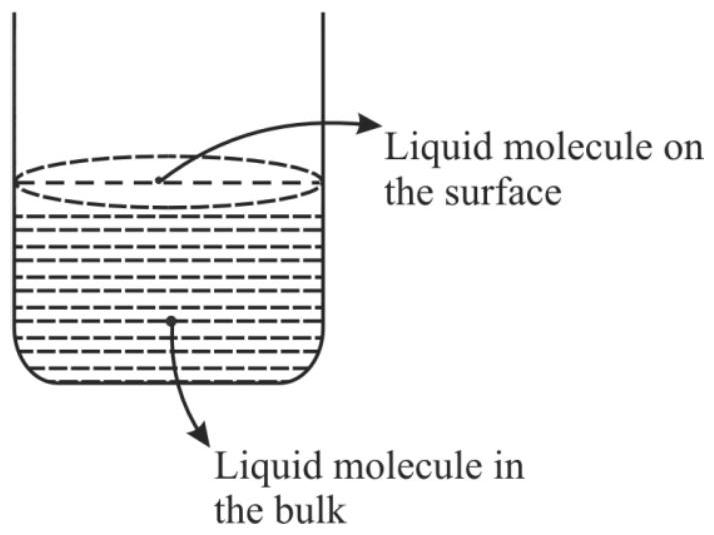
\includegraphics[max width=\textwidth, center]{2025_10_02_f0bf008abd968cf9b89ag-8}\\
A. Surface tension is the outcome of equal attractive and repulsion forces acting on the liquid molecule in bulk.\\
B. Surface tension is due to uneven forces acting on the molecules present on the surface.\\
C. The molecule in the bulk can never come to the liquid surface.\\
D. The molecules on the surface are responsible for vapour pressure if the system is a closed system.

Official Ans. by NTA (2.00)\\
Allen Ans. (2.00)\\
Sol. B and D options are correct.\\
59. A first order reaction has the rate constant, \(\mathrm{k}=4.6 \times 10^{-3} \mathrm{~s}^{-1}\). The number of correct statement/s from the following is/are \(\_\_\_\_\) .

Given : \(\log 3=0.48\)\\
A. Reaction completes in 1000 s .\\
B. The reaction has a half-life of 500 s .\\
C. The time required for \(10 \%\) completion is 25 times the time required for \(90 \%\) completion.\\
D. The degree of dissociation is equal to \(\left(1-\mathrm{e}^{-\mathrm{kt}}\right)\).\\
E. The rate and the rate constant have the same unit.

Official Ans. by NTA (2.00)\\
Allen Ans. (2.00)\\
Sol. \(\quad \mathrm{t}_{10 \%}=\frac{1}{\mathrm{~K}} \ln \left(\frac{\mathrm{a}}{\mathrm{a}-\mathrm{x}}\right)=\frac{1}{\mathrm{~K}} \ln \left(\frac{100}{90}\right)\)\\
\(\mathrm{t}_{10 \%}=\frac{2.303}{\mathrm{~K}}(\log 10-\log 9)\)\\
\(\mathrm{t}_{10 \%}=\frac{2.093}{\mathrm{~K}} \times(0.04)\)\\
Similarly

\[
\begin{aligned}
& t_{90 \%}=\frac{1}{K} \ln \left(\frac{100}{10}\right) \\
& t_{90 \%}=\frac{2.303}{K} \\
& \frac{t_{90 \%}}{t_{10 \%}}=\frac{1}{0.04}=25 \\
& e^{k t}=\frac{a}{a-x} \\
& \frac{a-x}{a}=e^{-k t} \\
& 1-\frac{x}{a}=e^{-k t} \\
& x=a\left(1-e^{-k t}\right) \\
& \alpha=\frac{x}{a}=\left(1-e^{-k t}\right)
\end{aligned}
\]

\begin{enumerate}
  \setcounter{enumi}{59}
  \item The number of incorrect statement/s from the following is/are \(\_\_\_\_\)\\
A. Water vapours are adsorbed by anhydrous calcium chloride.\\
B. There is a decrease in surface energy during adsorption.\\
C. As the adsorption proceeds, \(\Delta \mathrm{H}\) becomes more and more negative.\\
D. Adsorption is accompanied by decrease in entropy of the system.
\end{enumerate}

Official Ans. by NTA (2.00)\\
Allen Ans. (2.00)\\
Sol. 'A' water vapours are absorbed by calcium chloride.\\
C. As the adsorption proceeds, \(\Delta \mathrm{H}\) becomes less and less negative.


\end{document}